% !TeX spellcheck = <none>
\documentclass[11pt,titlepage]{article}

\usepackage[french,american]{babel}
\usepackage[utf8]{inputenc}
\usepackage[T1]{fontenc}
\usepackage{lmodern}
\usepackage{amsmath,amsfonts,amssymb}
\usepackage{graphicx}
\usepackage[a4paper]{geometry}           % See geometry.pdf to learn the layout
%\geometry{landscape}                    % Activate for for rotated page 
                                         % geometry
%\usepackage[parfill]{parskip}           % Activate to begin paragraphs with an
                                         % empty line rather than an indent
\usepackage{graphicx}
\usepackage{amssymb}
\usepackage{epstopdf}
\usepackage{color}
\usepackage[tt]{titlepic}
\usepackage{fancyhdr}
\usepackage{secdot}
\usepackage{booktabs}
\usepackage{rotating}

% WD41, LRS/EPFL/PSI ----------------------------------------------------------
\usepackage{multirow}
\usepackage{tabularx}
\usepackage{ragged2e}                      % for '\RaggedRight' macro 
                                           % (allows hyphenation)
\newcolumntype{Y}{>{\RaggedRight\arraybackslash}X}
\usepackage[style=ieee, backend=bibtex]{biblatex}
\usepackage{courier}
\usepackage{caption}
\usepackage{pdfpages}
% Itemize under table
% from: http://tex.stackexchange.com/questions/150492/how-to-use-itemize-in-table-environment
\usepackage{booktabs}% http://ctan.org/pkg/booktabs
\newcommand{\tabitem}{~~\llap{\textbullet}~~}
\usepackage{enumitem}
\usepackage{array}
\usepackage{rotating}
\bibliography{report_2015.bib}
% -----------------------------------------------------------------------------


\topmargin=-0.45in      
%\evensidemargin=0in     
\oddsidemargin=-0.1in      
\textwidth=6.8in        
\textheight=9.0in     
%\headsep=0.25in         

% Titlepage -------------------------------------------------------------------
\DeclareGraphicsRule{.tif}{png}{.png}{`convert #1 `dirname #1`/`basename #1 .tif`.png}
\titlepic{
\includegraphics[width=17cm]{figures/research_plan_pic.pdf}}

\title{\textbf{Annual progress report \textcolor{blue}{2015}}}     %Change Year

\author{\large{\textbf{Damar Wicaksono} }\\\\
\large{\textbf{Prof. Andreas Pautz}} \\\
\large{\textbf{Omar Zerkak}} \\\\\\\
\Large{\textbf{Bayesian Uncertainty Quantification}} \\\\
\Large\textbf{of Physical Models} \\\\
\Large\textbf{in Thermal-Hydraulics System Code}}

\date{03.12.2015}				       %activate to remove date
% -----------------------------------------------------------------------------

\begin{document}

\maketitle

% 2nd Page, Epmty Page --------------------------------------------------------
\pagestyle{empty}
\clearpage\mbox{}\clearpage
% -----------------------------------------------------------------------------

% Top Header ------------------------------------------------------------------
\pagestyle{fancy} \pagenumbering{arabic} \setcounter{page}{1}
\addtolength{\headheight}{\baselineskip}
\newcommand{\ffont}{\fontsize{8}{8}\selectfont}
\lhead{ECOLE DOCTORALE\\ \textit{DOCTORAL SCHOOL}}
\chead{PROGRAMME DOCTORAL EN PHYSIQUE\\ \textit{DOCTORAL PROGRAM IN PHYSICS}}
\rhead{\bfseries\ffont  
\includegraphics[width=55pt]{figures/EPFL_LOG.pdf}}
\renewcommand{\headrulewidth}{0.4pt}
% -----------------------------------------------------------------------------
%\textcolor{white}.

\section{Objectives of research}

The objective of the research is to quantify the uncertainty of
physical model parameters implemented in a thermal-hydraulics system code.
The physical models concerned are the ones describing
the phasic interaction (heat and momentum exchange) in a complex
multiphase flow during reactor transient especially for the
\textit{reflood} phase following a loss-of-coolant-accident.
These models are parameterized either by  physical or empirical tuning 
parameters which values are uncertain.

Conforming with the practice of statistical uncertainty propagation widely
adopted in the field of nuclear engineering, probability theory is used to
quantify the uncertainties related to each one of these parameters in a form 
of density function and/or its approximation.
The derivation of this density is posed as an inverse statistical problem
following a bayesian approach as the parameters themselves are not directly
observable.
To this end, a methodology to quantify model uncertainty will be
developed combining probabilistic modeling with available relevant
experimental data taken from various separate effect test facilities.

\section{Work achieved in the past year (state of research)}

\subsection{Global Sensitivity Analysis Methodology for TRACE Reflood Model}

Following the LRS at PSI successfull participation in the OECD/NEA PREMIUM Phase IV Benchmark, where the uncertainty of reflood model parameters in TRACE code were propagated in a blind exercise, the question was posed on how the uncertain parameters are actually affecting the clad temperature prediction during a reflood transient.
This question stimulated the development of a sensitivity analysis methodology for TRACE at the LRS.
The goal of the analysis was to understand the reflood model behavior better through the exploration of the parameter space.
Specifically, it was to quantify \emph{how} and \emph{to what extent} the model output is affected by \emph{simultaneous inputs variations across their range of uncertainties}.
The emphasis on simultaneous variations accross range of uncertainties set a \emph{global} method, that is being adopted in the current development, apart from a \emph{local} one.

The aforementioned goals can be met by decomposing the output variance and computing a set of \emph{global sensitivity} measures. 
These indices, quantify the contribution of the inputs variances to the output variance.
The work achieved during the year focused on the main-effect and total-effect indices.
They quantify the effect of a single parameter variation alone and its total interaction with the other parameters, respectively.
An interacting model is considered to be more complex as it complicates the task of parameter calibration or uncertainty reduction.

This paradigm of \textit{variance-based global sensitivity measure} particulary fits well with the current practice of uncertainty propagation in nuclear engineering thermal-hydraulics simulation.
Following the practice, for a given simulation case, sets of uncertain input parameters values are randomly generated and simultaneously perturbed, and the code is then evaluated multiple times using
these randomly generated points in parameter space.
The dispersion (i.e., variance) of the prediction is summarized and reported to establish a notion of reliability in the prediction.
The global method of sensitivity complements this uncertainty analysis by quantifying the 
aforementioned questions of \emph{how} and \emph{to what extent} input variations affect the output.

The choice of model output of interest is an important initial step in a sensitivity analysis. Its choice is guided by the selected goal.
In the spirit of model exploration, a more descriptive metric had to be derived to quantify the overall reflood curves variations.
Such description is not straightforward as the curves variations often showed complitaed change in shape stemming from concurrent variation in phase as well as in amplitude (See Fig.~\ref{fig:output}(a) for an illustration).
To tackle such problem, a method based on Functional Data Analysis (FDA) framework was applied.
By applying a \emph{time-warping} transformation, the convoluted phase-amplitude variations were first separated. Then by applying the Karhunen - Lo\`eve (KL) transformation, a few modes of variation were extracted (See Fig.~\ref{fig:output}(b)).
A set of scalar model outputs of interest was then finally derived whic parsimoniously described the overall functional variation of a reflood curves dataset, defined over the time domain.
Preliminary work on the application of FDA for the analysis of reflood simulation was presented at the NUTHOS-10 conference on last December and subsequently included in the proceeding \cite{Wicaksono2014a}.

\begin{figure}[h!]
	\centering
		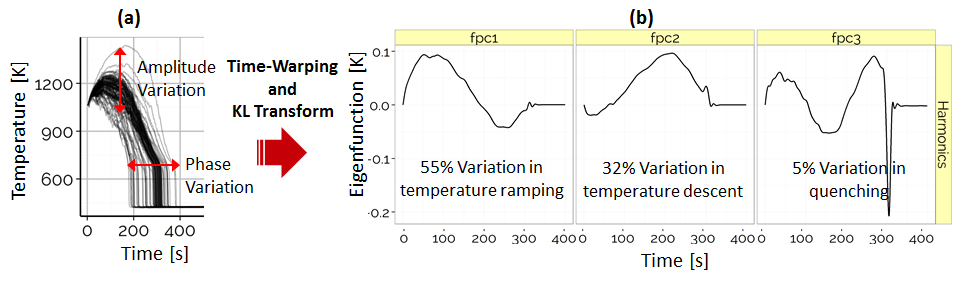
\includegraphics[scale=0.65]{figures/modelOutputsOfInterest.png}
	\caption{\textbf{(a)} A typical reflood simulation outputs from uncertainty propagations; \textbf{(b)} Three modes of variations extracted from the reflood curves by using FDA framework}
	\label{fig:output}
\end{figure}

The computation of Sobol' indices involved integrations in high-dimensional input parameter space.
These integrals are estimated by Monte Carlo sampling, equipped with an efficient estimator and a space-filling experimental design.
It is required that TRACE code to be evaluated at various input values.
As the number of code runs (thus computing time) is proportional to number of input parameters, screening analysis using the cheaper Morris method was conducted to screen out non-influential input parameters. It was found that only 10 out of 26 initial inputs were considered to be influential for the temperature transient (shown left). 
These parameters were mainly related to the Dispersed Film Flow Boiling (DFFB) and the spacer grid heat transfer models.
Fig.~\ref{fig:influential} gives an illustration regarding the notion of \emph{influential} parameters.
This implementation and application of the Morris method was also presented at the NUTHOS-10 conference last December\cite{Wicaksono2014b}.
The paper was subsequently awarded one of the best student paper award.

\begin{figure}[h!]
	\centering
	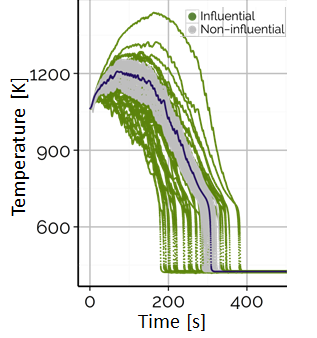
\includegraphics[scale=0.65]{figures/influentialRuns.png}
	\caption{Output variations from uncertainty propagation calculation due to 10 influential parameters (green) vs. 16 non-influential ones (gray)}
	\label{fig:influential}
\end{figure}

A result on variance decomposition on the reduced parameter space is shown in Fig.~\ref{fig:1stpc}.
The TRACE Reflood model was found to relatively additive and non-interacting.
Also, the output variation can be attributed only to a small set of parameters related to the spacer grid and DFFB models. 
The finding were not contrary to the currently held expert judgment on these parameteres importance.
Yet, the analysis was able to \emph{make precise} this judgment quantitatively, demonstrating the value of the method.
The result was presented at the NURETH-16 conference \cite{Wicaksono2015a} and selected as one of the best student papers.

\begin{figure}[h!]
	\centering
	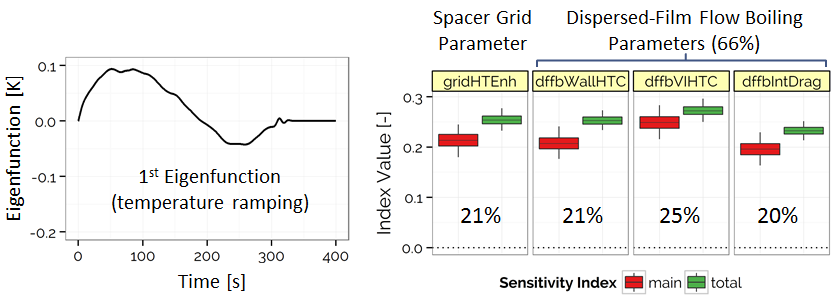
\includegraphics[scale=0.65]{figures/1stPrincipalComponent.png}
	\caption{The decomposition of $1^\textnormal{st}$-principal component describing the variation in temperature ramping; the sum of main-effect indices of $92\%$ indicates a non-interacting model}
	\label{fig:1stpc}
\end{figure}

Nevertheless, when considering the $2^\textnormal{nd}$-principal component, only $32\%$ of the variation is due to the main effect, indicating that parameters interactions are responsible for the variation in the temperature descent phase.
This might become an issue when the parameters have to be calibrated against experimental data around this region because multiple combination of parameters value would yield the same fit.
The structure of this interaction, however, remains unclear.
Therefore, the logical next step is to reveal this structure and a method to estimate $2^\textnormal{nd}$-order sensitivity indices is being implemented to that end.

\begin{figure}[h!]
	\centering
	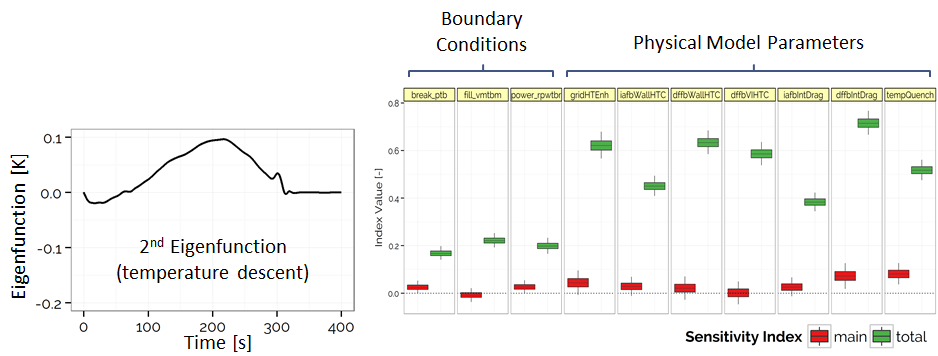
\includegraphics[scale=0.65]{figures/2ndPrincipalComponent.png}
	\caption{The decomposition of $2^\textnormal{nd}$-principal component describing the variation in temperature ramping; the sum of main-effect indices of $32\%$ and large difference between the main- and total-effect indices, indicate a highly interacting model}
	\label{fig:2ndpc}
\end{figure}

\subsection{Generation of Reflood Facility TRACE Model from CAD Processing Tool} 

The sensitivity of the solution to the adopted nodalization scheme is a longstanding issue in system thermal-hydraulics modelling.
Through nodalization, a complex geometry of a thermal-hydraulic system is practically simplified into a set of interconnected \emph{nodes}. 
A node is a discretized element defined by its length and free volume. 
At its faces, a node is also defined by flow areas and hydraulic diameter (see Fig.~\ref{fig:nodalization}).

As the analysists are usually given a great flexibility in developing their own nodalization scheme, a situation where multiple nodalization schemes of the same system due to \textit{ad hoc} choices give very different prediction of system behavior might arise (the so-called user effect).
Though best-practice suggestions exist, the solution verification can only be empirically established by comparing several nodalization scheme to check how sensitive the prediction is and to exclude (or at least minimized) the user-effect in the model qualification process.

\begin{figure}[h!]
	\centering
	\includegraphics[scale=0.65]{figures/nodalization.png}
	\caption{Representation of a nuclear power plant as a network of interconnected and simplified \emph{nodes}}
	\label{fig:nodalization}
\end{figure}

The adopted approach to develop nodalization in this PhD project so far was using spreadsheet. 
Though easy to set up initially, it becomes cumbersome and error prone, especially if several nodalization schemes are to be prepared.
An additional activity was thus carried out to develop a pre-processing tool to generate a TRACE model (input deck) directly from a solid model constructed in SolidWorks software.
This project is part of the outstanding research activity in LRS at PSI whose long-term goal is to be able to generate a TRACE input model of a complex plant in 3-Dimension directly out of CAD model.
This CAD (solid) model is usually constructed with higher fidelity from the available drawing.
The currently available, but disconnected scripting tools written in VBA (Visual Basic for Application, VBA) from previous activities are consolidated and written using fully-featured programming language of Visual Basic .NET.
The tool is also implemented as an object-oriented program to ease further development to extend its capabilities.

For the purpose of the present PhD project, however, the aim is simply to have a working 
version for the development of a simple reflood facility model, 
a 1-dimensional (axial).
Based on a simple boolean algebra operation on the solid model 
(also known as Constructive Solid Geometry, CSG), the tool is able to 
extract relevant fluid information from the solid to construct the set of nodes.
As an extension from the previous development, relevant information related to
a heat structure (for a rod and slab geometry) can also be generated directly 
from the solid model. 
All the extracted relevant information serve as a basis to generate a TRACE input deck. 

\pagebreak

\section{Current state of work}

The current state of research during the year are summarized in 
Table~\ref{tab:currentstate} shown below.

\begin{table}[h!]
	\caption{Current state of research in relation to the original
		(1\textsuperscript{st} year) work plan
	}
	\label{tab:currentstate}
	\begin{center}
		\footnotesize
		\begin{tabular}{c l l l}
% Header ----------------------------------------------------------------------
			\toprule[1.5pt]
			Phase 
			& Task Description 
			& Planned Outcome 
			& Current State of Work \\ \hline
% 1st Element -----------------------------------------------------------------
			\textbf{1} 
			& \parbox[c]{0.3\textwidth}{%
				Comprehensive reviews of post-CHF flow closure             %Task Description
				laws in TRACE and externalization of important
				model parameters} 
			& \parbox[c]{0.2\textwidth}{
				1 Technical Report} 
			& \parbox[c]{0.3\textwidth}{%
				\begin{itemize}[leftmargin=1em,itemsep=1pt,parsep=0pt]\raggedright%
					\item Important reflood model parameters externalized
					\item PSI contribution to OECD/NEA PREMIUM Benchmark finalized
				\end{itemize}} \\ \hline
% 2nd Element -----------------------------------------------------------------
				\textbf{2} 
				& \parbox[c]{0.3\textwidth}{%
					Global sensitivity analysis (GSA) based on FEBA test facility}  
				& \parbox[c]{0.2\textwidth}{%
					\begin{itemize}[leftmargin=1em,itemsep=1pt,parsep=0pt]\raggedright%
						\item 1 Technical report
						\item 1 Journal article
					\end{itemize}}
				& \parbox[c]{0.3\textwidth}{%
					\begin{itemize}[leftmargin=1em,itemsep=1pt,parsep=0pt]\raggedright%
						\item A paper on Morris method presented at NUTHOS-10
						\item A paper on FDA application presented at NUTHOS-10
						\item A paper on GSA methodology presented at NURETH-16
						\item A manuscript on GSA for submission to NSE (\textit{under preparation})
						\item A technical report on nodalization studies (\textit{under preparation})
					\end{itemize}} \\ \hline
% 3rd Element -----------------------------------------------------------------
				\textbf{3} 
				& \parbox[c]{0.3\textwidth}{
					\begin{itemize}[leftmargin=1em,itemsep=1pt,parsep=0pt]\raggedright%
						\item Definition of error and probabilistic error model
						\item Calibration of TRACE reflood model based on the FEBA facility
						\item Approximation of the posterior distribution by Markov-Chain Monte Carlo
					\end{itemize}}
				& \parbox[c]{0.2\textwidth}{%
					\begin{itemize}[leftmargin=1em,itemsep=1pt,parsep=0pt]\raggedright%
						\item 1 Technical report
						\item 1 Journal article
						\item 1 Conference article
					\end{itemize}}
				& \parbox[c]{0.3\textwidth}{
					Abstract to be submitted to NUTHOS-11 (\textit{under preparation})} \\	\hline
% 4th Element -----------------------------------------------------------------
				\textbf{4} 
				& \parbox[c]{0.3\textwidth}{
					\begin{itemize}[leftmargin=1em,itemsep=1pt,parsep=0pt]\raggedright%
						\item Calibration of TRACE reflood model based on other reflood test facility
						\item Consolidation of the calibration results based on 2 facilities and validation based on another reflood test facility
					\end{itemize}}
				& \parbox[c]{0.2\textwidth}{%
					\begin{itemize}[leftmargin=1em,itemsep=1pt,parsep=0pt]\raggedright%
						\item 1 journal article
					\end{itemize}} 
				& \parbox[c]{0.3\textwidth}{%
					\begin{itemize}[leftmargin=1em,itemsep=1pt,parsep=0pt]\raggedright%
						\item \textbf{Task redefined}: calibration will only based on FEBA, validation will be done against ACHILLES test facility
						\item Scripting based on VB.NET has been developed to assist in input deck 		
							  generation
						\item ACHILLES test facility model in TRACE is currently being developed as part of M.Sc. student's work
					\end{itemize}}\\ \hline
% 5th Element -----------------------------------------------------------------
				\textbf{5} 
				& \parbox[c]{0.2\textwidth}{
					Thesis-Write Up}
				& \parbox[c]{0.2\textwidth}{%
					Thesis} 
				& \multicolumn{1}{c}{$-$}\\ 
% End --------------------------------------------------------------------------
			\bottomrule[1.5pt]
		\end{tabular}
	\end{center}
\end{table}
				
The work on global sensitivity analysis (GSA) for reflood model in TRACE took the most 
of the available time during the year 2015. 
A paper contribution on the variance decomposition coupled with functional data analysis method was
presented at the NURETH-16 conference.
The results presented in the paper, for the first time in the analysis of reflood model,:
\begin{enumerate}
	\item \emph{Confirmed} expert judgment on parameters relative 
	importance (namely, the parameters related to Dispersed Film Flow Boiling model)
	\item \emph{Made precise} the importance in quantitative manner (namely, in terms of variance decomposition of functional components)
	\item \emph{Revealed} additional model behavior that was overlooked (namely, strong parameter interactions during the temperature descent of reflood transient)
\end{enumerate}
All the work related to the global sensitivity analysis methodology done so far 
is being finalized and will be concluded with a submission to NSE journal publication 
for review (submission is due 01.2016).

The invitation to be considered in NSE publication from the NURETH-16 paper was not foreseen.
As such, this particular submission will be a minor revision to the conference paper complemented with
additional literature study, derivation of formula, elaboration of methodology, and additional
explanations; no additional results are planned to be added.
Following such scheme, a second paper on global sensitivity analysis of FEBA model with additional results, such as second-order sensitivity indices estimation and full set of FEBA experiments can be foreseen.

Consolidation of all the scripting works to carry out simulation experiment campaign is 
on-going.
The tools are implemented as Python packages, and currently being separated 
into two packages: \texttt{trace\_simexp} to manage TRACE runs in large Monte Carlo 
simulation campaign and  \texttt{gsa\_module} a more generic package to generate design 
matrix, compute quantities of interest, and compute sensitivity measures 
(based on Morris and Sobol').
The tools are designed to enforce reproducibility with explicit parameterization for options and
built based on open-source libraries of \texttt{Python} and \texttt{R}.

Additional work on the development of a pre-processing tool 
for direct generation of TRACE model from a CAD model was also done during the same period.
The tool can be used to assist in developing a nodalization scheme of a 1D 
reflood facility model.
The tool is currently being tested both for FEBA and ACHILLES test facilities, of which 
the latter is carried out as part of an M.Sc. student's work.
A technical report on nodalization studies of FEBA model is currently being prepared.

\section{Calendar of upcoming work}

With the conclusion of GSA methodology development, a better understanding of the reflood model
as well as the elaboration of the parameters importance on the transient have been achieved.
The work will continue with the calibration of this model using the available experimental data.
First, error model will be defined probabilistically. Secondly, the prior distribution of the important model parameters will be updated and the posterior distribution will be approximated by using 
a Markov Chain Monte Carlo algorithm. 
Finally, validation will be done by propagating the updated parameters uncertainties on the
ACHILLES test facility model \emph{blindly}.
To initiate this part of the work, a review of various available error model and its probabilistic 
representations applicable for statistical calibration is being done as part of NUTHOS-11 conference
contribution. The upcoming works is planned following Fig.~\ref{fig:calendar}.

\begin{figure}[h!]
	\centering
	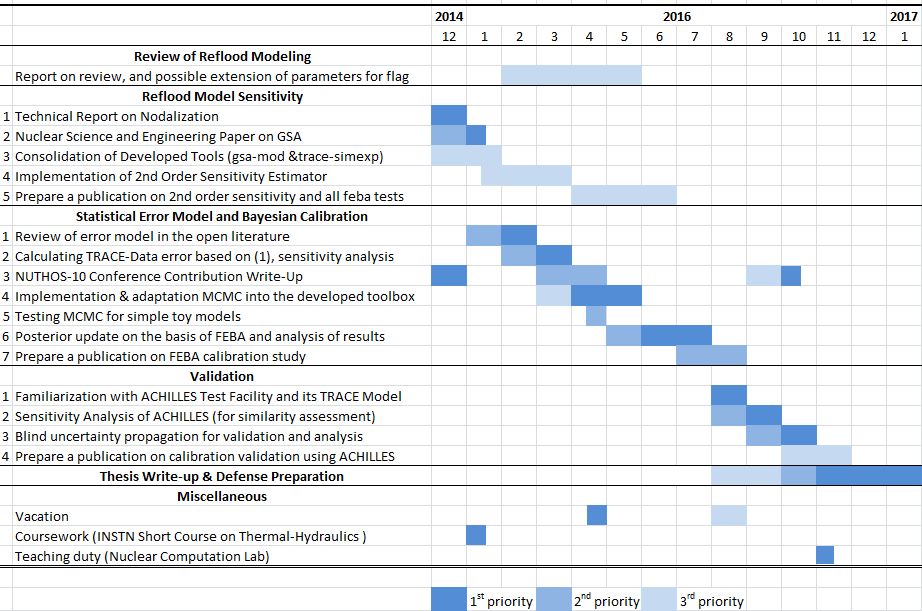
\includegraphics[scale=0.60]{figures/calendar.png}
	\caption{Calendar of upcoming works}
	\label{fig:calendar}
\end{figure}

\section{Other activities and remarks}

\subsection{Nuclear Computation Lab (ETH-531)}

A teaching activity was carried out for a part of the Nuclear Computation Lab 
course organized at PSI (one chapter, entitled ``Basic Thermal-hydraulics'', out of 
6 chapters in total). 
The course is part of the EPFL/ETHZ Nuclear Engineering Master Program and has 
now become an obligatory course for students.
A single day was dedicated for a lecture session followed by a hands-on computer
simulation session using the TRACE code.
Seventeen students participated in the course this semester (5 additional students 
compared to the previous year)

The simulation session this year was extended to add an additional exercise.
The resulting 3 short simulations are now built around a central theme of 
the basic \emph{limiting phenomena} in nuclear power plant transient: 
critical flow, counter-current limitation, and critical heat flux (CHF).
A time was allocated to prepare the course documentation and hands-on notes 
\cite{Wicaksono2015c}, as well as testing the simulation environment.
The students managed to do a good work and have a better average 
scores overall compared to the previous batches of students. 

\section{Scientific publications, conference contributions, and presentations}

\nocite{Wicaksono2014a}
\nocite{Wicaksono2014b}
\nocite{Wicaksono2015a}
\nocite{Wicaksono2015b}
\nocite{Wicaksono2015c}

\printbibliography[heading=none]

%% Signature Page
%\newpage
%%\textcolor{white}.\\\\
%\noindent\textbf{Comments by the thesis advisor(s)}\\\\
%\noindent\textbf{Prof. A Pautz}\\\\
%............................................................................
%............................................................................\\\
%............................................................................
%............................................................................\\\
%............................................................................
%............................................................................\\\
%............................................................................
%............................................................................\\\
%............................................................................
%............................................................................\\\
%............................................................................
%............................................................................\\\
%............................................................................
%............................................................................\\\
%............................................................................
%............................................................................\\\
%............................................................................
%............................................................................\\\
%
%\noindent\textbf{O. Zerkak}\\\\
%\noindent Damar can be credited with a prolific and promising first phase of his research 
%project. 
%Despite unavoidable initial difficulties, Damar could assimilate the 
%topic and rapidly become independent.
%He proposed a solution approach of his own, that he will need to implement and 
%test for the reflood problem next year.
%His approach of combining FDA with a solution method for Bayesian inference 
%problem (such as Markov Chain Monte Carlo sampling) is very original in 
%the nuclear engineering field.
%I should also add that Damar has proved very reliable in executing PSI 
%contribution to the OECD/NEA PREMIUM project.
%
%\section*{\underline{Signatures}\\}
%\noindent \textbf{Thesis advisor}\hspace{6.25cm}\dotfill\vspace{0.5cm}\\
%
%\noindent \textbf{Thesis co-advisor}\hspace{5.7cm}\dotfill\\
%\noindent  (if officially nominated)\\\\
%
%\noindent \textbf{With his signature, the candidate confirms that he took note 
%                  of the above comments.}\\\\
%
%\noindent \textbf{Candidate}\hspace{7cm}\dotfill\vspace{0.5cm}\\
%
%\noindent \textbf{Date}\hspace{8.05cm}\dotfill\\
%
%\vspace{0.8cm}
%%\begin{center}
%%\textbf{Up to 5 pages in total}
%%\end{center}
%\begin{center}
%\textbf{To be returned to:} \textcolor{green}{EPFL-EDPY / Station 3 
%                                              / 1015 Lausanne / Suisse}
%\end{center}

% Directly attached signed form
%
\includepdf[pages={1}]{figures/Planned-Signed-ZO41.pdf}

\end{document}
